\chapter{Системийн зохиомж}

\begin{figure}[h]
  \centering
  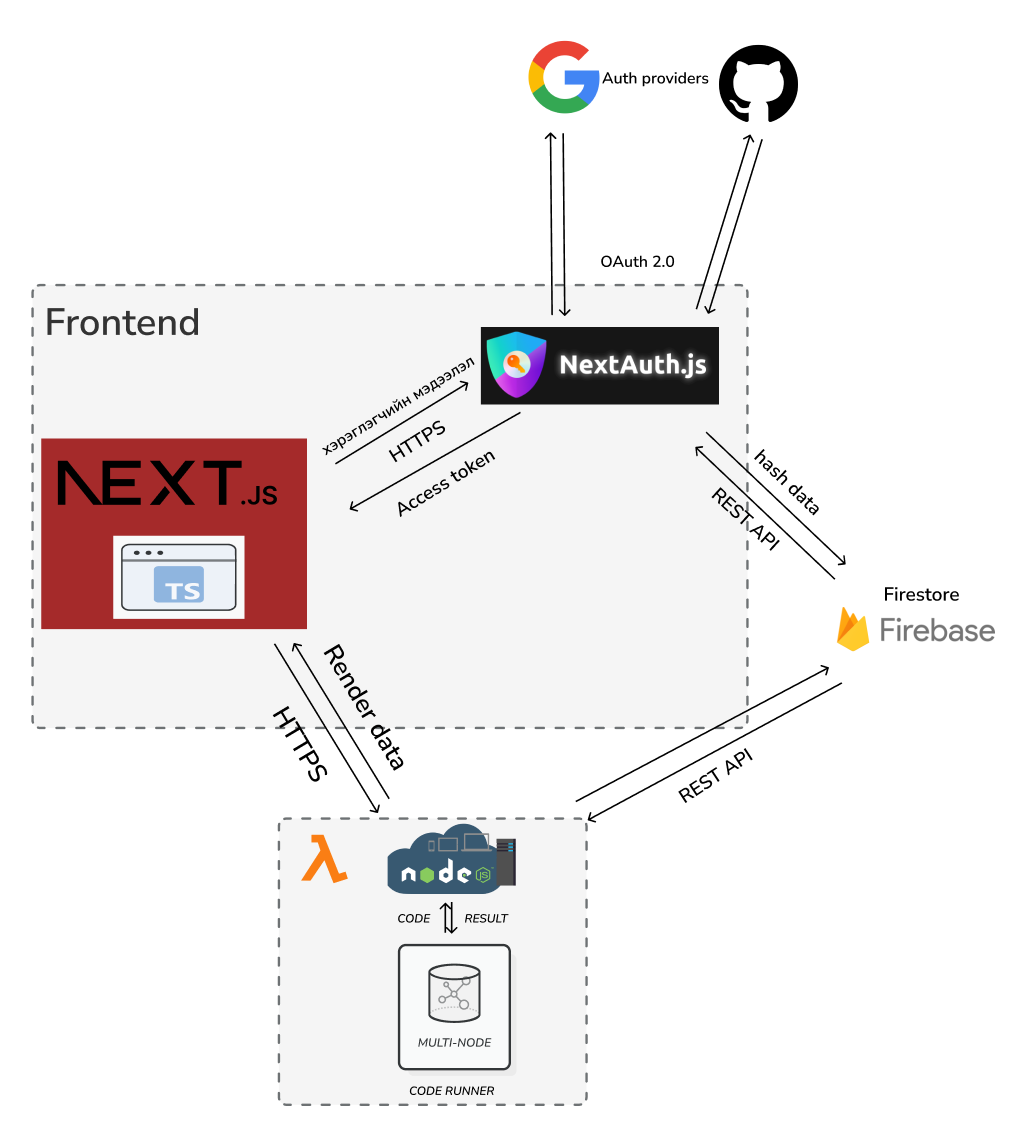
\includegraphics{img/diagrams/architecture.PNG}
  \caption{Системийн ерөнхий зураглал}
\end{figure}

"Coldbrains" системийн ашиглаж буй технологиуд болон тэдгээрийн холбоог харуулж байгаа бөгөөд аль болох ерөнхий байдлаар дүрслэхийг оролдов.

\clearpage

\section{Хэрэглэгчийн интерфейс}
\subsection{Wireframe}
\begin{figure}[h]
  \centering
  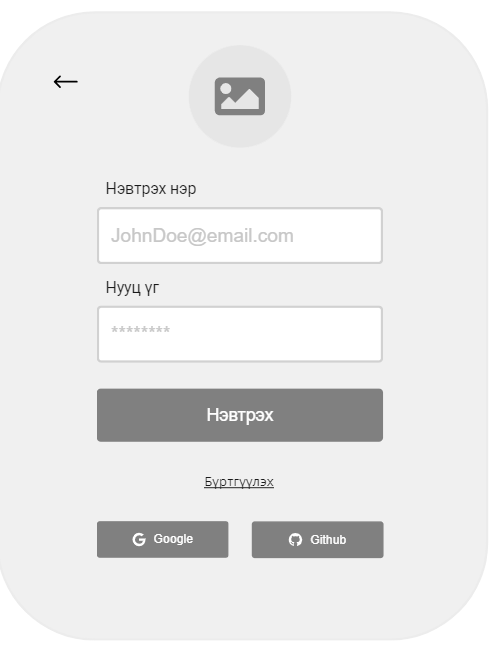
\includegraphics[width=5cm]{img/wireframe/login.PNG}
  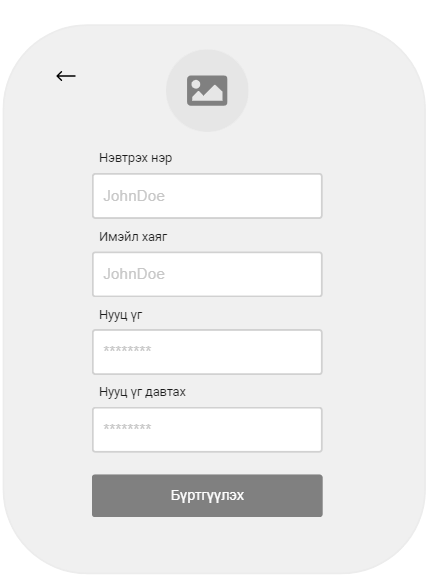
\includegraphics[width=5cm]{img/wireframe/register.PNG}
  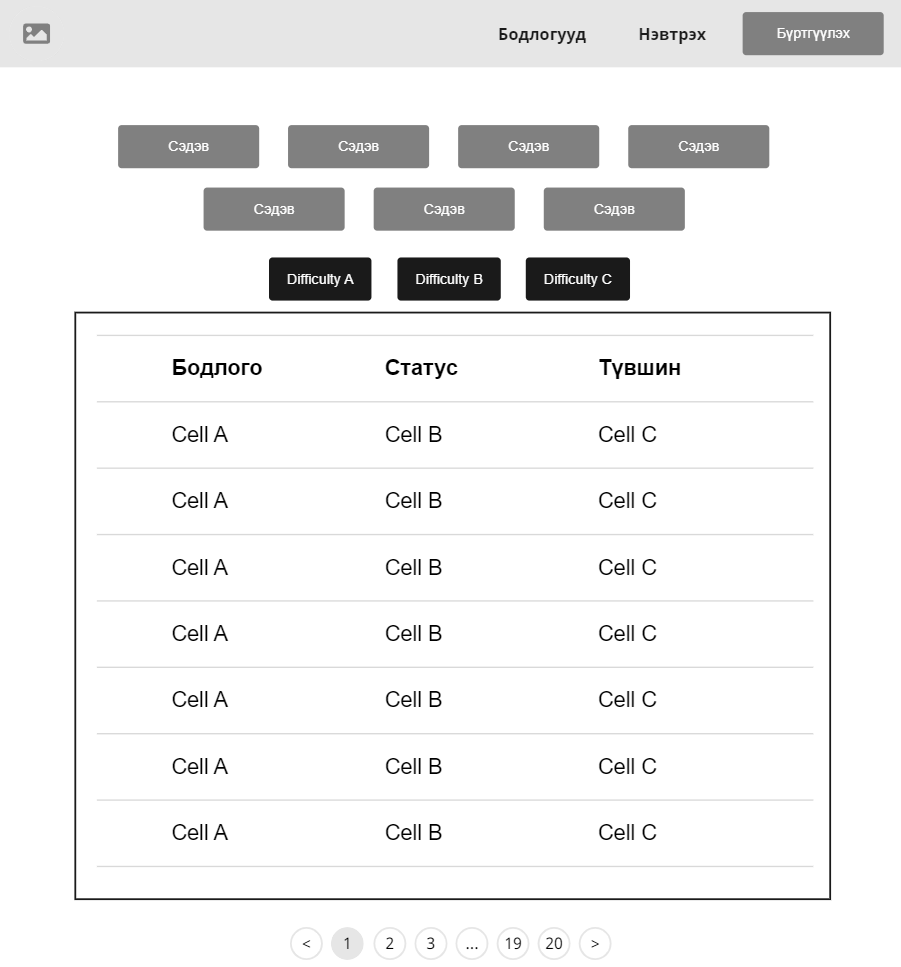
\includegraphics[width=5cm]{img/wireframe/problems.PNG}
  \caption{Wireframe}
\end{figure}

\subsection{Mockup дизайн}
\begin{figure}[h]
  \centering
  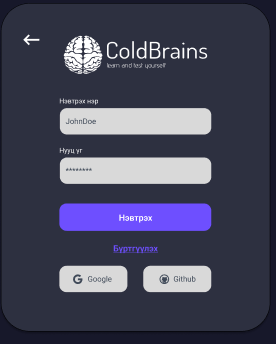
\includegraphics[width=5cm]{img/mockup/login.PNG}
  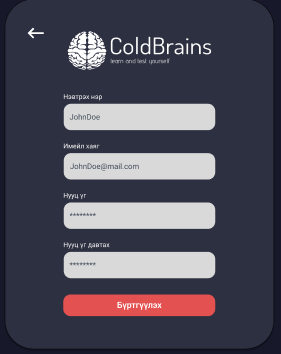
\includegraphics[width=5cm]{img/mockup/register.PNG}
  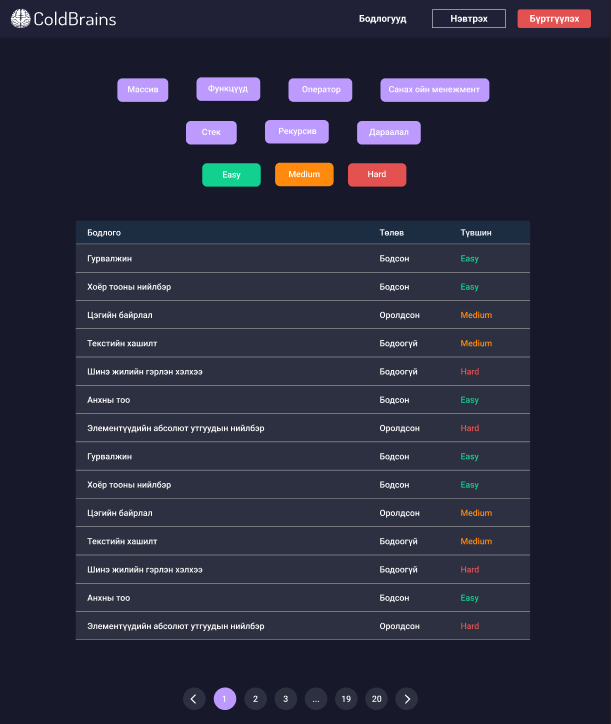
\includegraphics[width=5cm]{img/mockup/problems.PNG}
  \caption{Mockup}
\end{figure}

\clearpage

Wireframe-ийг илүү дэлгэрэнгүй \cite{wireframe}-с харах боломжтой. Нэвтрэх, бүртгүүлэх, бодлогууд, профайл, бодолт, хариунууд, хариу зэрэг интерфейсүүдийг зохиомжилсон.

Өнгөний сонголтуудыг \textbf{Visual Studio Code} код засварлагчийн хамгийн түгээмэл сонголтууд\cite{VSC theme} болон \textbf{Programming Color Palette}-ээс сэдэвлэн оноож өгсөн билээ.

\section{Технологиуд болон шийдлүүд}
\subsection{NEXTjs хувилбар 13}
NEXTjs нь React сангийн фреймворк бөгөөд хамгийн түгээмэл хэрэглэгддэг интерактив фреймворк юм. Хэрэглэгчийн интерфейсийг хэрэгжүүлэхэд хамгийн өргөн сонголтууд болон том экосистем\footnotemark{}тэйгээрээ бусад технологиудаасаа илүү байж чаддаг билээ.\footnotetext{Тухайн технологитой холбоо бүхий мэдээлэл, хэрэглээний бодит жишээ, заах арга зүйн нэгдэл} NEXTjs-ийн тусламжтайгаар хэрэглэгчийн интерфейсийг интерактив олон компонентуудад хувааж, хэрэглэгчийн үйл ажиллагааг хянах боломжтой. 

NEXTjs-ийн хувилбар 13-ыг ашигласнаар дата дамжуулах болон сервер талдаа компонентуудыг зурах, cache хийх аргачлал зэрэг илүү хөгжүүлэгчид хялбар байх бөгөөд маш олон түгээмэл ашиглагддаг сан, package-ууд нь NEXTjs/React-д зориулан нийтлэгдсэн байдаг.

\subsection{Next.js auth}
Энэхүү сан нь NEXTjs дээр \textbf{session control} хийхэд хамгийн тохиромжтой бөгөөд хэрэглэгчид зориулсан JWT(Json Web Token) токеныг бэлдэж cookie дээр байршуулж, мөн гадны олон түгээмэл системүүдтэй хэрэглэгчийн нээлттэй датаг хуваалцах боломжийг олгодог. Үүний Google, Github зэрэг мэдээллээр хангагчтай харьцах боломж бүхий хэсгийг NEXTjs дээр амархан ашиглах боломжтой. Хэрэглэгчийн нэвтрэх токенг cookie байдлаар хадгалж тухайн токеноос хэрэглэгчийн мэдээллийг decrypt хийж ашиглах боломжоор хангаж өгдөг. 

\subsection{MUI дизайн}
Material UI нь Google-ийн Material дизайныг хэрэгжүүлдэг React компонентуудын сан юм. Интерфейс хэрэгжүүлдэг frontend инженерүүдийн хувьд цагийг хэмнэсэн түгээмэл багаж бөгөөд React-ийн \textbf{Server Side Rendering}-ийг дэмждэг билээ. 

Цаашлаад богино хугацаанд өөрийн өнгөний загварчилгаа(customization) бүхий Responsive интерфейсийг хэрэгжүүлэхэд тусалдаг билээ. Одоогоор React-ийн хамгийн олон хэрэглэгчтэй сан гэж тодорхойлогддог билээ. 

\subsection{Codemirror}
Codemirror гэх энэхүү javascript UI(хэрэглэгчийн интерфейс) бүхий сан нь "Coldbrains"-д гол тоглогчийн үүргийг гүйцэтгэж байгаа бөгөөд энэхүү сангийн тухай дурьдвал
7 хоног бүр 2-3 сая гаруй таталттай байдаг.   

\begin{figure}[h]
  \centering
  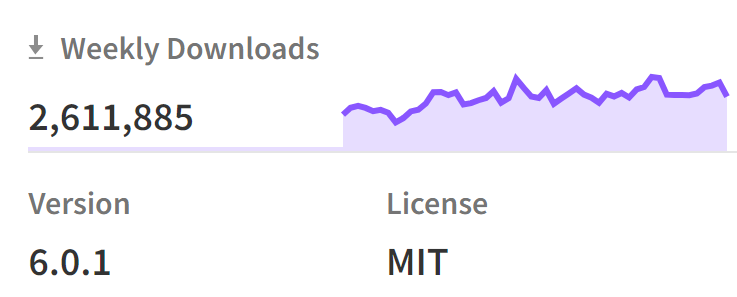
\includegraphics{img/codemirror-npm.PNG}
  \caption{Codemirror сан}
\end{figure}

Цаашлаад Microsoft-ийн Monaco Editor(Visual Studio Code дээр ашиглагддаг), Tern.js зэрэг сангуудын туслажтайгаар Intellisense бүхий код засварлагчийг бий болгох боломжтой бөгөөд өөрөө тухайн код бичигчдээ зориулан extension\footnotemark{} \footnotetext{Боломжит өргөтгөл}-үүдийг бичиг өгөх боломжтой бөгөөд олон төрлийн платформуудыг дэмждэг билээ. 

"Coldbrains" систем дээр энэхүү Codemirror сан нь маш хэрэгтэй хэрэглэгчийн интерфейсийн үүргийг гүйцэтгэж байгаа бөгөөд Codemirror сан дээр бичсэн uiw/react-codemirror сан нь энэхүү хэрэглээг илүү уян хатан болгож, олон хэлний синтакс болон олон өнгөний сонголт зэрэг боломжуудыг бий болгож байгаа. Код засварлагчийн болон хэрэглэгчийн интерфейсийг уян хатан байдлаар хэрэгжүүлэхэд энэхүү \hyperlink{https://uiwjs.github.io/react-codemirror/}{@uiw/codemirror} шийдэл болж байгаа.

\subsection{AWS болон Firebase}
Хэрэглэгчийн кодыг функциональ програмчлалын аргаар зохиомжлогдсон сервер дээр ажиллуулах бөгөөд энэ нь AWS-ийн Lambda буюу stateless байдлаар ажилладаг серверт тохиромжтой. AWS нь тухайн хүсэлтийг хүлээж аван тодорхой холбоо үүсгэх ба handshake хийлгүйгээр REST API-аар Firebase-ийн Firestore NoSQL өгөгдлийн сан руу дата дамжуулах билээ. 

AWS lambda нь хүсэлт ирэх үед хамгийн хурдан хариу өгөхийн тулд Cold start\footnotemark{} \footnotetext{Эхнээс нь бүр мөсөн асаах} хийхээс сэргийлж хамгийн сүүлд ажиллагаатай байсан container-ийг ашигладаг бөгөөд тухайн container-ууд ажиллагаанд ороогүй удсан тохиолдолд нөөцийг хэмнэн өөрийн санах ойг цэвэрлэдэг байна. 

Singapore дээр байрлах серверийг ашигласан болно. Firestore 50000 уншилт/сар, 20000 бичилт/сард үнэгүй ашиглах боломжийг олгодог. AWS lambda нь мөн адил бөгөөд MVP(Minimum viable product)-ийг хэрэгжүүлэхэд эдгээр платформууд нь хамгийн тохиромжтой гэж үзсэн.

\subsection{Хэрэглэгчийн кодыг ажиллуулах}
Хэрэглэгчийн кодыг хэл тус бүр дээр аюулгүй ажиллагаан үүднээс AWS-ийн lambda серверийг ашиглаж байгаа. Эдгээр нь
\begin{enumerate}
  \item Python - python-shell
  \item C/C++ - emscripten
  \item Javascript - javascript virtual machine 2
\end{enumerate}
зэрэг сан болон технологиудыг кодыг ажиллуулахаар ашигласан байгаа билээ. Эдгээр нь customizable буюу оролт/гаралт, ашиглах боломжтой сангууд, ажиллах хугацааны хязгаарлалтуудыг тус тус дэмждэг бөгөөд AWS lambda сервер дээр байршуулснаар тухайн серверийн нөөцийн хуваарилалтыг шийдэж өгч байгаа билээ. 

\subsection{Bcrypt}
\subsection{ExpressJS}
\subsection{...}